\chapter{Numerical Results}

The validation tables and numerical figures in this chapter are generated by
the review scripts described in Chapter 4; the phase-check table and figure
come from the separate dispersion check. Decimal strings such as
\texttt{1.0e-03} mean \(10^{-3}\). Full CSV data and solver timings are
available in \path{submission/assets/tables/}; raw run logs, VTUs and
diagnostics remain in \path{output/validation/review/}.

\section{Spatial Refinement}
The following are absolute displacement errors at \(T=1\), with
\(h=\sqrt{2}/N\), \(Q_1\), and \(\Delta t=0.00125\).
Orders are computed between successive meshes, not fitted from time curves.
\begin{center}\small
\begin{tabular}{llllll}
\toprule
case & N & $L^2$ & $H^1$ & $p_{L^2}$ & $p_{H^1}$\\
\midrule
free & 12 & 7.58223066e-03 & 5.40023915e-02 & - & -\\
free & 24 & 1.90327194e-03 & 2.36042082e-02 & 1.9941 & 1.1940\\
free & 48 & 4.72437969e-04 & 1.13323955e-02 & 2.0103 & 1.0586\\
forced & 12 & 5.94615919e-03 & 1.68258681e-01 & - & -\\
forced & 24 & 1.49397989e-03 & 8.39901647e-02 & 1.9928 & 1.0024\\
forced & 48 & 3.73329003e-04 & 4.19772495e-02 & 2.0006 & 1.0006\\
\bottomrule
\end{tabular}\end{center}


\begin{figure}[H]
 \centering
 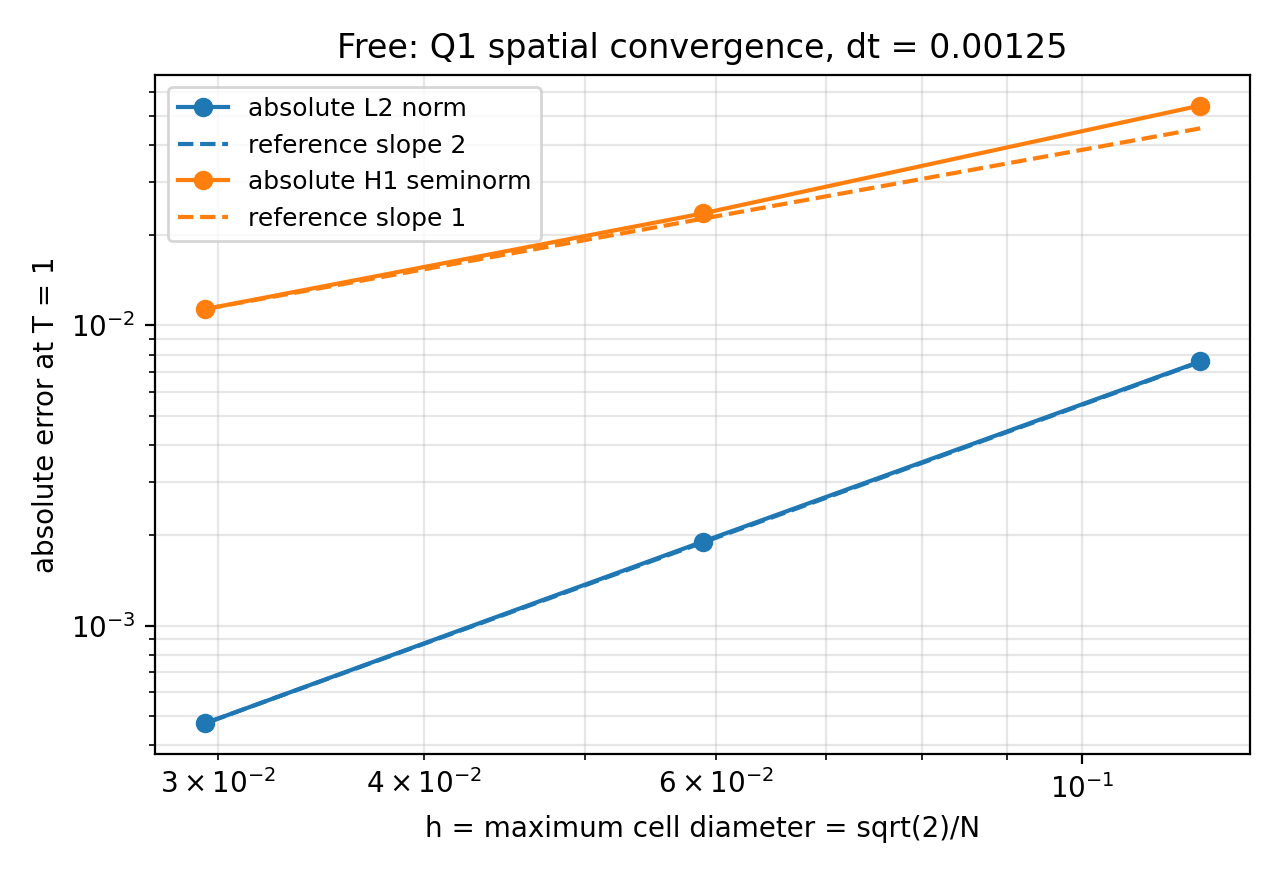
\includegraphics[width=0.82\textwidth]{../../assets/figures/free-convergence.png}
 \caption{Free solution: final absolute spatial errors versus maximum cell
 diameter on log--log axes. Dashed lines show Q1 reference slopes.}
\end{figure}
\begin{figure}[H]
 \centering
 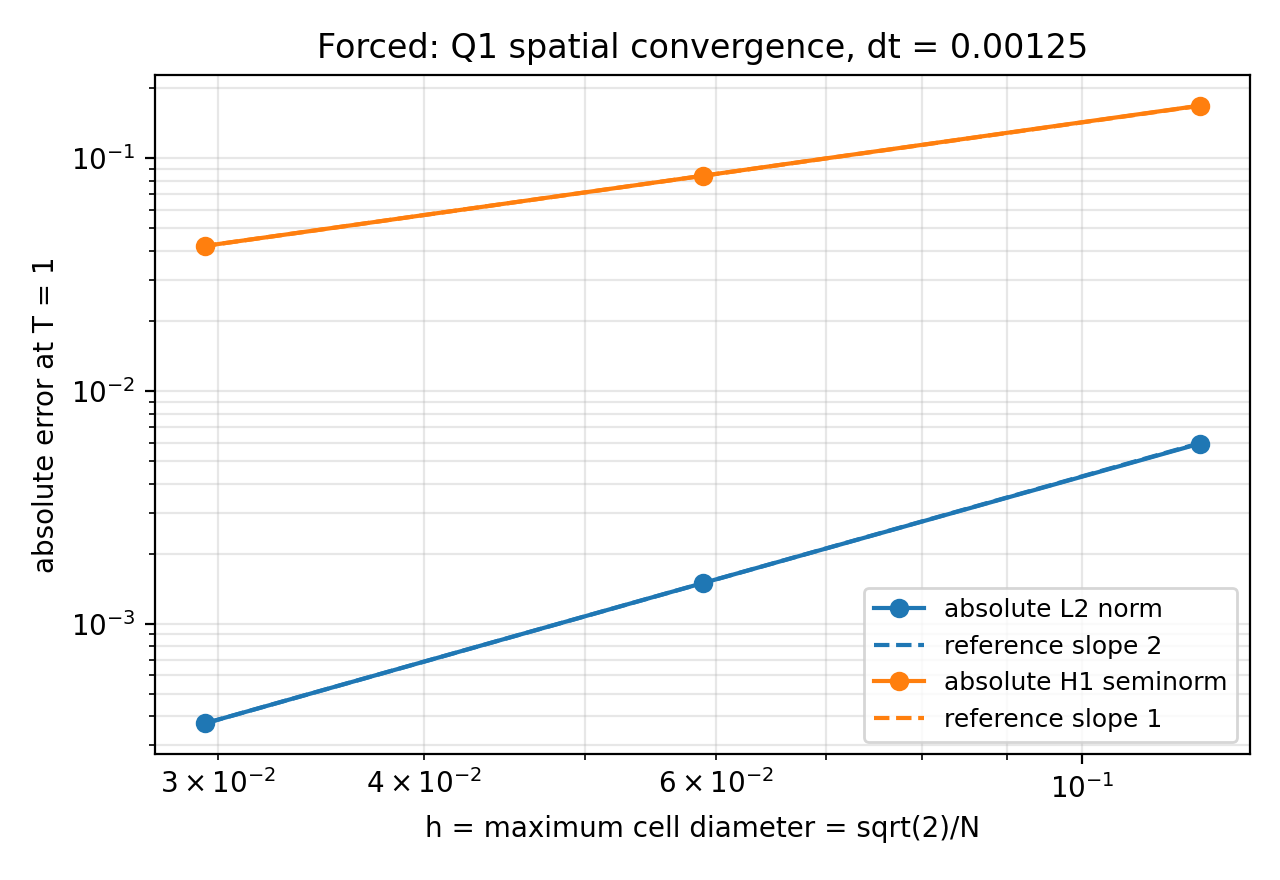
\includegraphics[width=0.82\textwidth]{../../assets/figures/forced-convergence.png}
 \caption{Forced solution: the same mesh-convergence experiment and norm
 definitions. These are not error-versus-time curves.}
\end{figure}

\section{Temporal Contamination Check}
For each mesh we halve \(\Delta t\) from 0.00125 to 0.000625, keeping
\(T=1\). The table reports
\(\left|e_{\Delta t/2}-e_{\Delta t}\right|/e_{\Delta t}\) for each final
error norm. The small changes support interpreting the mesh experiment as
predominantly spatial. They do not prove a rigorous bound on temporal error.
\begin{center}\small
\begin{tabular}{llll}
\toprule
case & N & $L^2$ change & $H^1$ change\\
\midrule
free & 12 & 5.435649e-04 & 1.914659e-04\\
free & 24 & 2.164670e-03 & 2.506564e-04\\
free & 48 & 8.719531e-03 & 2.703558e-04\\
forced & 12 & 1.124933e-04 & 1.386920e-06\\
forced & 24 & 4.504379e-04 & 1.406438e-06\\
forced & 48 & 1.804992e-03 & 1.408030e-06\\
\bottomrule
\end{tabular}\end{center}


The older validation suite uses \(\Delta t=0.0025\) for spatial refinement.
Its fixed-\(N=32\) tests at \(\Delta t=0.02,0.01,0.005\) mix spatial and temporal
errors. In particular, cancellation can make the total error increase as
the time step decreases. Those results are preserved in
\texttt{validation-summary.md} and are not presented as measured temporal
order. Second-order Newmark accuracy here is a theoretical property of the
scheme.

\section{Empirical Phase Check}
The phase formula in Chapter 3 can also be examined directly. We record the
displacement at the centre of the square, where the manufactured free solution
has its largest amplitude, and estimate the first numerical maximum by a
quadratic interpolation of the three samples around the discrete peak. The
exact period is \(2\pi/(\sqrt{2}\pi)=\sqrt{2}\). The experiment uses
\(N=192\), so the spatial contribution is small compared with the coarser
meshes used in the convergence study.

\begin{center}
\small
\begin{tabular}{rrrrr}
\toprule
$\Delta t$ & exact period & numerical peak & peak lag & phase lag (rad) \\
\midrule
0.02000 & 1.41421356 & 1.41513027 & 9.16702662e-04 & 4.07280262e-03 \\
0.01000 & 1.41421356 & 1.41443023 & 2.16668199e-04 & 9.62631444e-04 \\
0.00500 & 1.41421356 & 1.41425597 & 4.24077963e-05 & 1.88412875e-04 \\
\bottomrule
\end{tabular}
\end{center}


\begin{figure}[H]
 \centering
 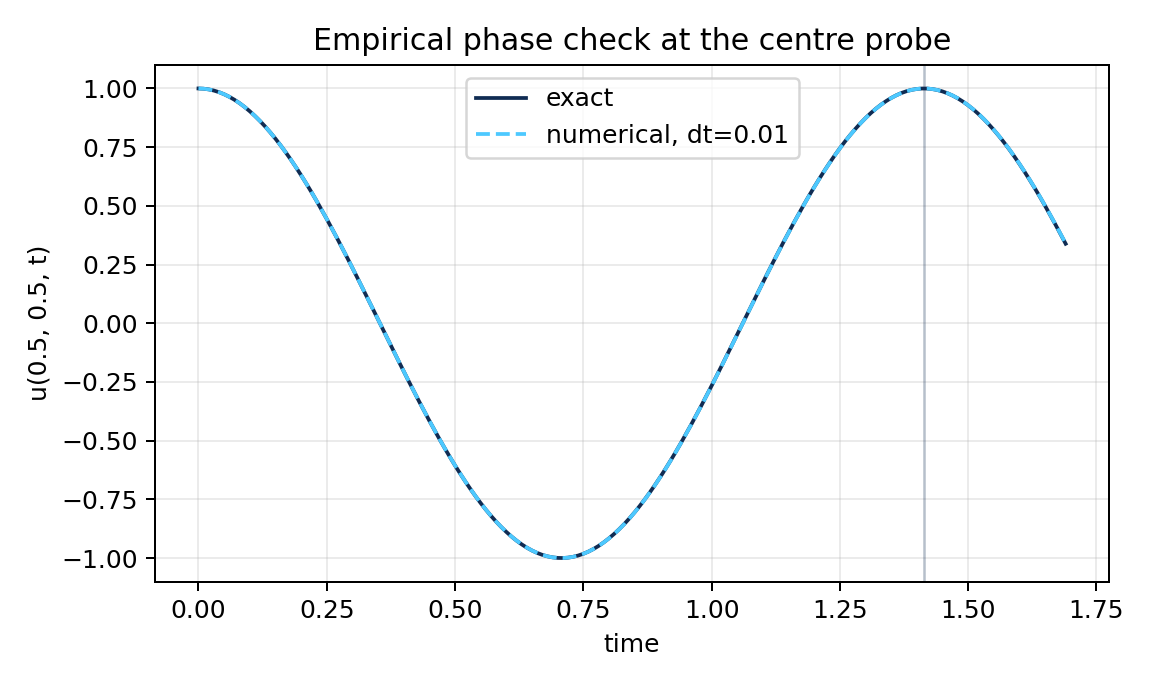
\includegraphics[width=0.78\textwidth]{../../assets/figures/dispersion-check.png}
 \caption{Centre-probe phase check for the free mode with \(\Delta t=0.01\).
 The numerical first peak is compared with the exact period; the vertical
 line marks the exact peak time.}
\end{figure}

The measured peak lag decreases from \(9.17\times10^{-4}\) to
\(4.24\times10^{-5}\) when the time step is reduced from \(0.02\) to \(0.005\),
consistent with the second-order phase error of average-acceleration Newmark.
The lag contains both spatial semi-discrete dispersion and temporal
dispersion, so this is an empirical consistency check rather than an isolated
measurement of temporal order.

\section{Error Evolution and Energy}
The following time curves use \(N=48\), \(Q_1\), \(\Delta t=0.00125\).
Each error sample is a spatial norm of the displacement error at that time.
Semilogarithmic vertical axes resolve small errors; the horizontal axis is
linear time.
\begin{figure}[H]
 \centering
 \begin{subfigure}{0.48\textwidth}
  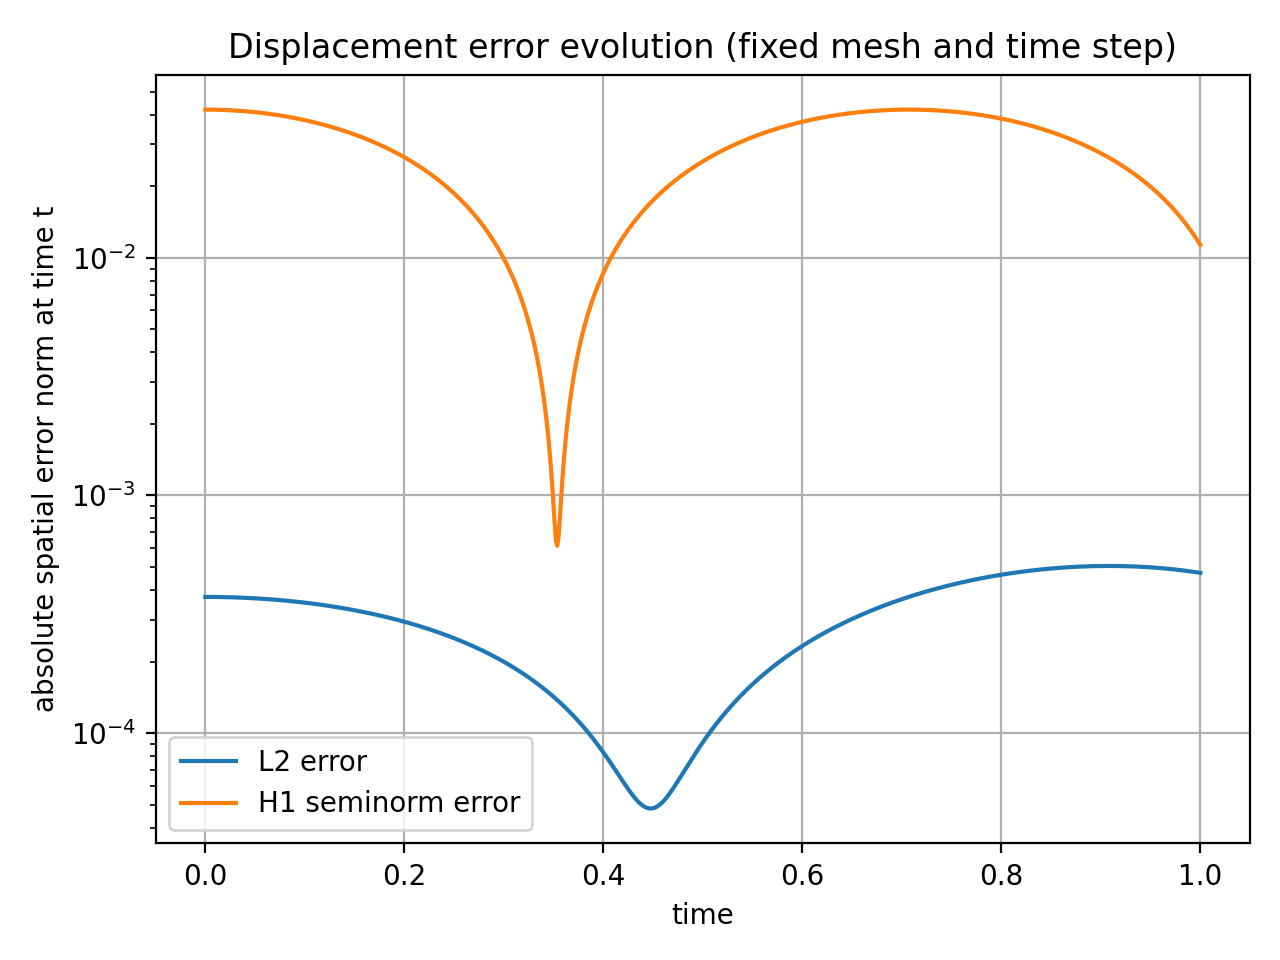
\includegraphics[width=\textwidth]{../../assets/figures/free-time-errors.png}
  \caption{Free: absolute errors versus time.}
 \end{subfigure}\hfill
 \begin{subfigure}{0.48\textwidth}
  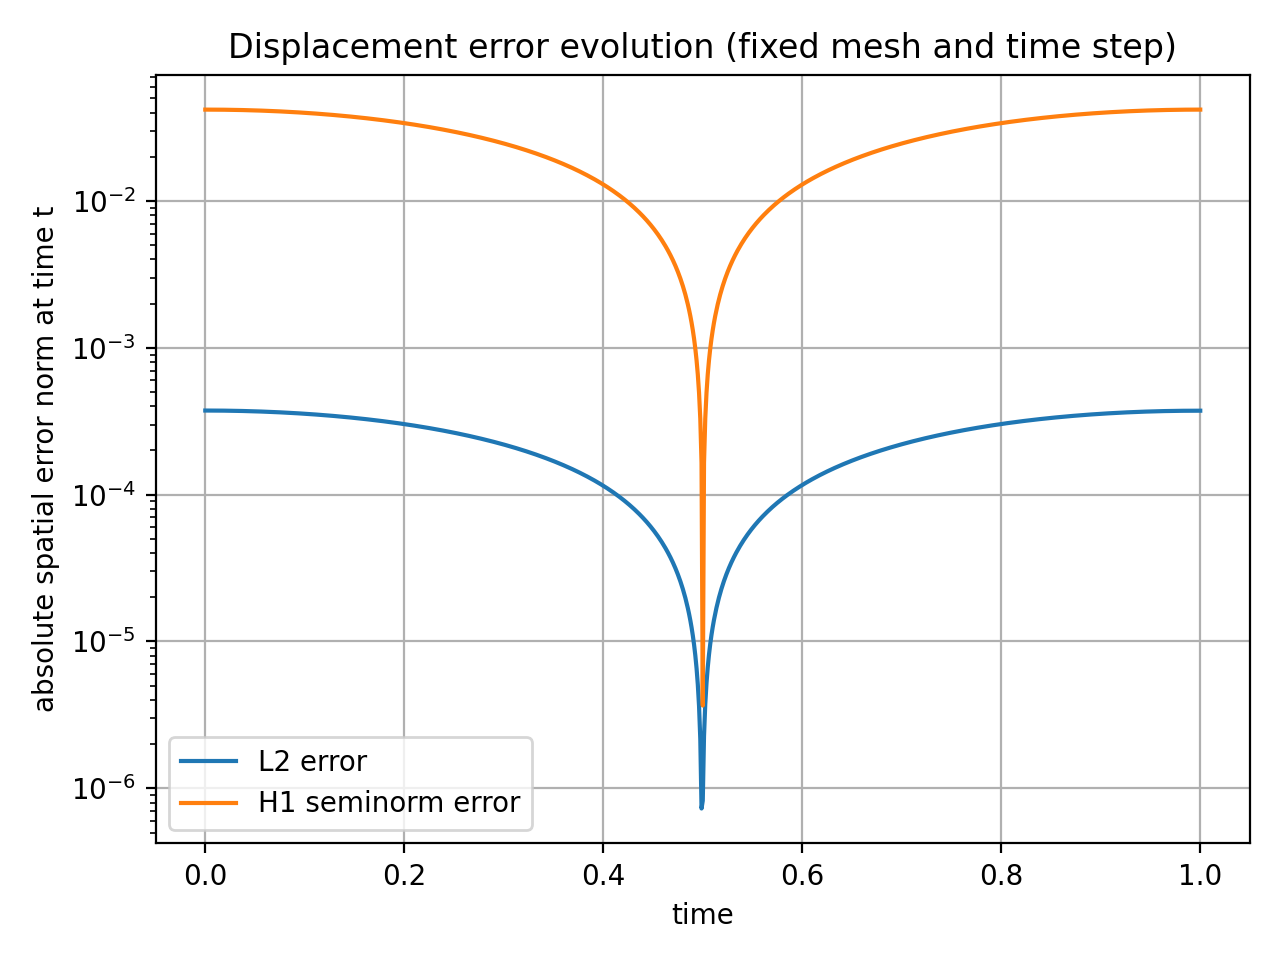
\includegraphics[width=\textwidth]{../../assets/figures/forced-time-errors.png}
  \caption{Forced: absolute errors versus time.}
 \end{subfigure}
 \caption{Time evolution on a fixed mesh, distinct from spatial convergence.}
\end{figure}

\begin{center}\small
\begin{tabular}{lllll}
\toprule
case & initial & final & minimum & max. rel. change\\
\midrule
free & 2.4647600926 & 2.4647600926 & 2.4647600926 & 5.225087e-15\\
forced & 2.4647600926 & 2.46476994554 & 1.23194254076 & 5.001775e-01\\
\bottomrule
\end{tabular}\end{center}

The last column is \(\max_n|E_h^n-E_h^0|/E_h^0\). It measures numerical drift
only for the free case. For the forced case it mainly measures physical
energy exchange. Energy is computed from the original \(M,K\); its initial
value differs slightly from the continuous \(\pi^2/4\) due to interpolation.

\begin{figure}[H]
 \centering
 \begin{subfigure}{0.48\textwidth}
  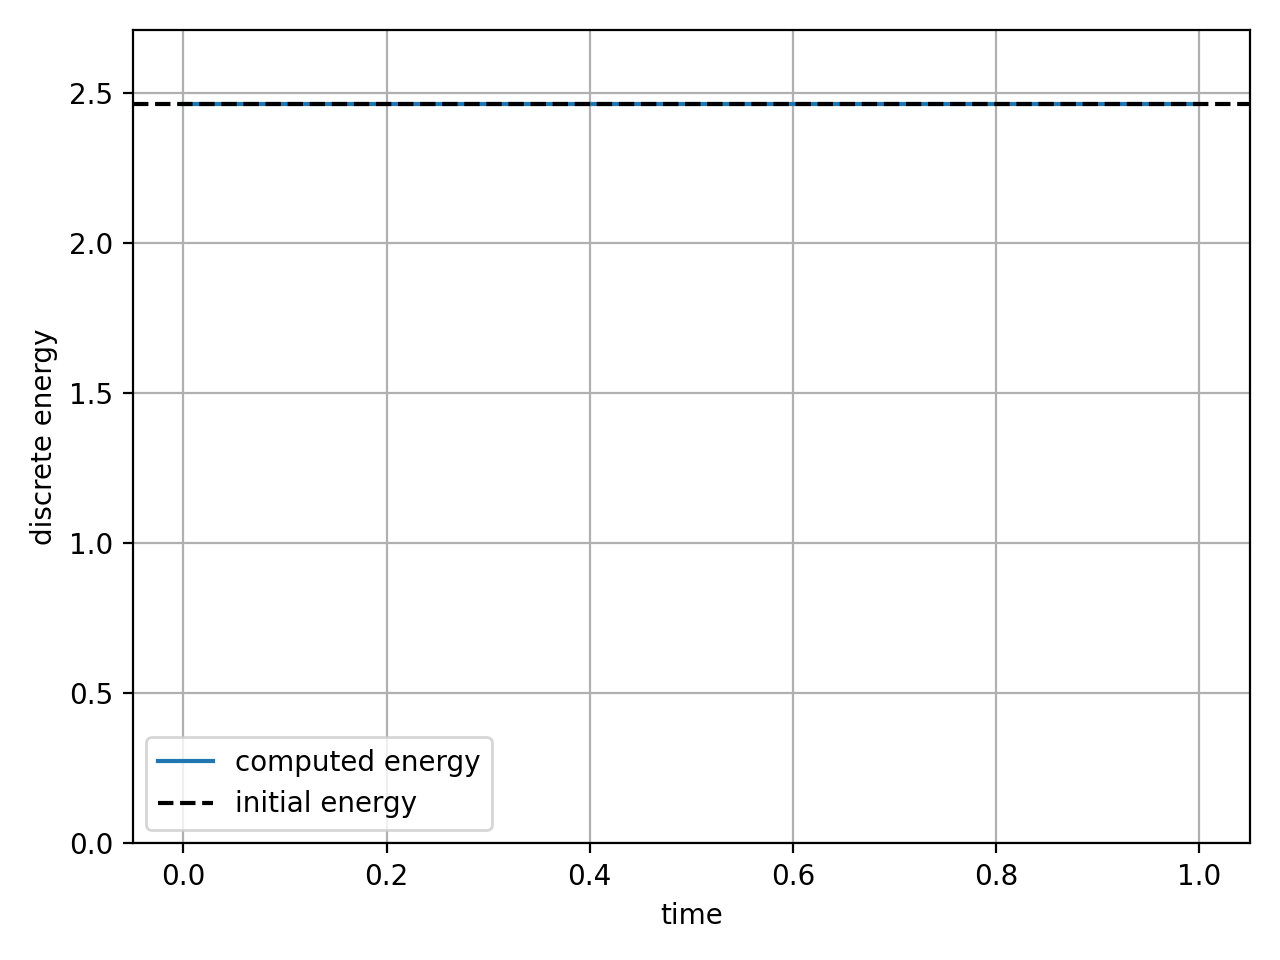
\includegraphics[width=\textwidth]{../../assets/figures/free-time-energy.png}
  \caption{Free mechanical energy.}
 \end{subfigure}\hfill
 \begin{subfigure}{0.48\textwidth}
  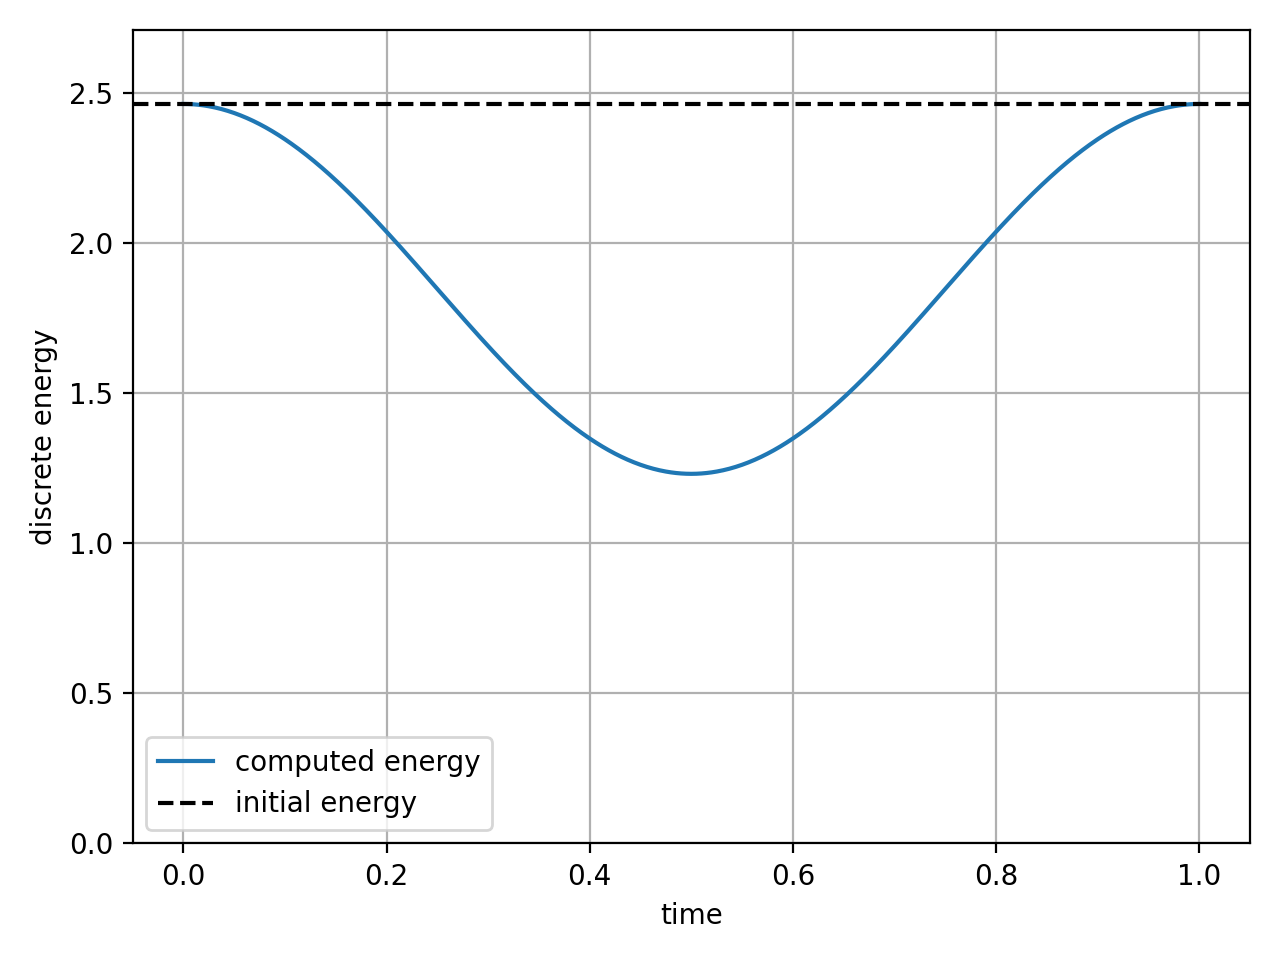
\includegraphics[width=\textwidth]{../../assets/figures/forced-time-energy.png}
  \caption{Forced mechanical energy.}
 \end{subfigure}
 \caption{Absolute energy with a zero baseline. Forcing removes and later
 returns energy; free energy is constant up to numerical error.}
\end{figure}
\begin{figure}[H]
 \centering
 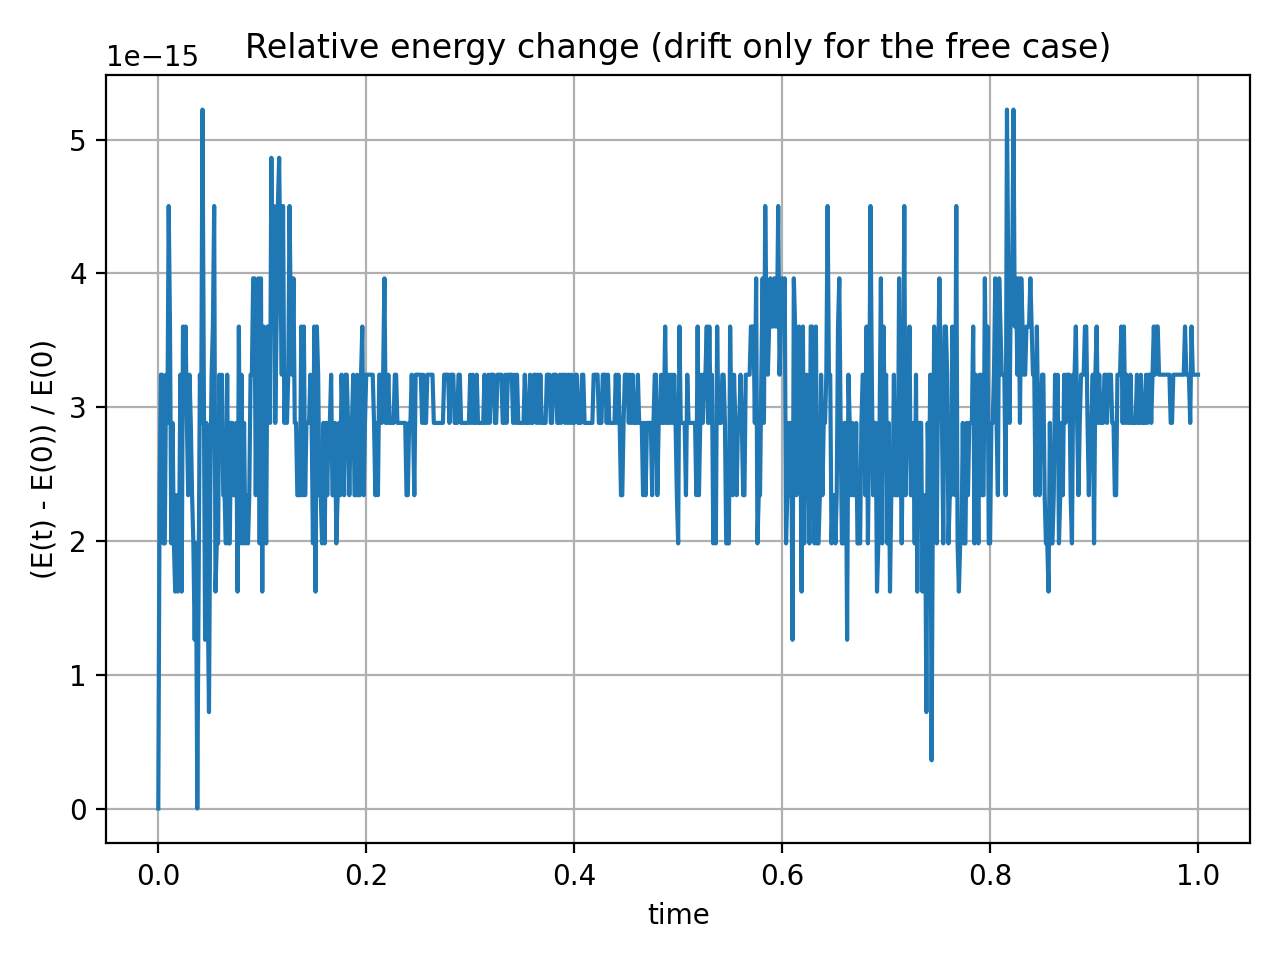
\includegraphics[width=0.78\textwidth]{../../assets/figures/free-time-energy_change.png}
 \caption{Free-case relative energy drift. The scale exposes small
 round-off/solver effects that are invisible on the absolute-energy plot.}
\end{figure}

\section{Solver Comparison}
All combinations solve the forced \(Q_1\), \(N=48\) problem (2401 stored
DoFs), \(T=0.1\), \(\Delta t=0.005\), on the same host in Release mode.
There are three repetitions per combination, all with the same stopping
tolerances and zero initial guesses. The initial mass solve is excluded
from this timing table. Mean iterations and maximum true residual are over
all 60 Newmark solves. Solve and preconditioner setup times are medians of
the totals for 20 time steps, in milliseconds. File output, assembly,
diagnostics and the independent residual recomputation are outside these timers.
\begin{center}\small
\begin{tabular}{lllllll}
\toprule
solver & prec. & converged & mean it. & max. residual & solve ms & setup ms\\
\midrule
cg & ssor & 3/3 & 6.00 & 2.615100e-12 & 29.87302 & 1.98151\\
cg & jacobi & 3/3 & 1.00 & 1.447179e-14 & 5.65763 & 0.06972\\
gmres & ssor & 3/3 & 6.00 & 2.605978e-12 & 44.73600 & 1.98325\\
gmres & jacobi & 3/3 & 1.00 & 1.425311e-14 & 6.06195 & 0.07157\\
\bottomrule
\end{tabular}\end{center}


All combinations agree in final errors and energy within relative tolerance
\(10^{-7}\) and absolute tolerance \(10^{-10}\). Sparse symmetry and
Rayleigh-quotient checks also pass; they supplement the SPD proof in Chapter 4.

Jacobi needs one iteration because the sine mode is an eigenvector of the
uniform-grid interior mass/stiffness operators and diagonal scaling preserves
it. SSOR need not preserve that eigenspace. This special result does not
predict general-load performance. CG+SSOR remains the baseline; timings are
machine-dependent and are not parallel scaling.
